\begin{subfigure}{0.6\textwidth}
	\centering
	\begin{tikzpicture}[scale=2.5]
		\coordinate(c1) at (-0.47943,0.87758);
		\coordinate(c2) at (-0.98278,-0.18477);
		\coordinate(c3) at (-0.12797,-0.99178);
		\coordinate(c4) at (0.90369,-0.42818);
		\coordinate(c5) at (0.68648,0.72715);
	\draw (c1) -- (c2) -- (c3) -- (c4) -- (c5) -- cycle;
		\draw[->] (-1.2,-1.3) -- (-0.2,-1.3);
		\draw[->] (-1.2,-1.3) -- (-1.2,-0.3);		\node(x) at (-0.1,-1.3) {\(x\)};
		\node(y) at (-1.2,-0.2) {\(y\)};
		
		\node(Si) at (0,0) {\(S_i\)};
	\end{tikzpicture}
	\caption{}\label{fig:p2polyhedrondecompositiona}
\end{subfigure}

\vspace{40pt}

\begin{subfigure}{0.6\textwidth}
	\centering
	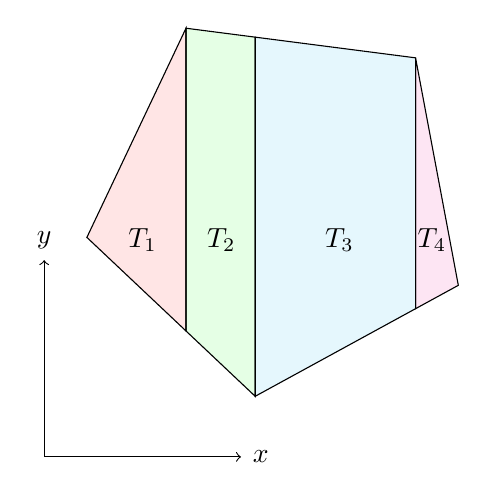
\begin{tikzpicture}[scale=2.5]
		\coordinate(c1) at (-0.98278,-0.18477);
		\coordinate(c2) at (-0.98278,-0.18477);
		\coordinate(c3) at (-0.47943,0.87758);
		\coordinate(c4) at (-0.47943,-0.65998);
		\filldraw[fill=red, fill opacity=0.1] (c1) -- (c2) -- (c3) -- (c4) -- cycle;
		\coordinate(c5) at (-0.47943,-0.65998);
		\coordinate(c6) at (-0.47943,0.87758);
		\coordinate(c7) at (-0.12797,0.83224);
		\coordinate(c8) at (-0.12797,-0.99178);
		\filldraw[fill=green, fill opacity=0.1] (c5) -- (c6) -- (c7) -- (c8) -- cycle;
		\coordinate(c9) at (-0.12797,-0.99178);
		\coordinate(c10) at (-0.12797,0.83224);
		\coordinate(c11) at (0.68648,0.72715);
		\coordinate(c12) at (0.68648,-0.54684);
		\filldraw[fill=cyan, fill opacity=0.1] (c9) -- (c10) -- (c11) -- (c12) -- cycle;
		\coordinate(c13) at (0.68648,-0.54684);
		\coordinate(c14) at (0.68648,0.72715);
		\coordinate(c15) at (0.90369,-0.42818);
		\coordinate(c16) at (0.90369,-0.42818);
		\filldraw[fill=magenta, fill opacity=0.1] (c13) -- (c14) -- (c15) -- (c16) -- cycle;
		\draw[->] (-1.2,-1.3) -- (-0.2,-1.3);
		\draw[->] (-1.2,-1.3) -- (-1.2,-0.3);		\node(x) at (-0.1,-1.3) {\(x\)};
		\node(y) at (-1.2,-0.2) {\(y\)};
		
		% Label trapezia
		\node(t1) at (-0.7,-0.2) {\(T_1\)};
		\node(t2) at (-0.3,-0.2) {\(T_2\)};
		\node(t3) at (0.3,-0.2) {\(T_3\)};
		\node(t4) at (0.77,-0.2) {\(T_4\)};
	\end{tikzpicture}
	\caption{}\label{fig:p2polyhedrondecompositionb}
\end{subfigure}
